\subsection{Analisis Pemilihan Teknologi Implementasi}

Proses penentuan teknologi untuk pembangunan sistem dalam penelitian ini mengalami beberapa tahapan evaluasi dan perubahan berdasarkan pertimbangan biaya, efisiensi, dan kebutuhan integrasi sistem.

\begin{enumerate}
    \item \textbf{Tahap awal (Google Cloud Platform)} \\
    Pada perencanaan awal, sistem dirancang untuk menggunakan layanan \textit{cloud} berbasis \textit{Google Cloud Platform} (GCP) mengingat kapabilitasnya yang kuat dalam manajemen data dan \textit{machine learning}. Namun, pendekatan ini tidak dilanjutkan karena faktor biaya operasional (\textit{cost}) yang tinggi dan kurang efisien untuk skala implementasi penelitian skripsi ini.

    \item \textbf{Tahap eksplorasi (Python dan Streamlit)} \\
    % Sebagai alternatif, penulis mengembangkan prototipe sistem menggunakan bahasa pemrograman \textbf{Python} dengan \textit{framework} \textbf{Streamlit}. Pemilihan ini didasarkan pada kemudahan Python dalam pengolahan data dan pembangunan model \textit{machine learning}. Meskipun prototipe ini berhasil berfungsi secara mandiri, ditemukan kendala signifikan dalam aspek interoperabilitas. Sistem berbasis Python sulit untuk diintegrasikan secara langsung dengan ekosistem aplikasi yang sedang dikembangkan oleh rekan mahasiswa lain dalam satu tim bimbingan.
    Sebagai alternatif awal, penulis mengembangkan prototipe sistem menggunakan bahasa pemrograman \textbf{Python} dengan \textit{framework} \textbf{Streamlit}. Pemilihan ini didasarkan pada kemudahan Python dalam pengolahan data dan pembangunan model \textit{machine learning}. Meskipun prototipe ini berhasil berfungsi secara mandiri, ditemukan kendala signifikan dalam aspek interoperabilitas. Sistem berbasis Python sulit untuk diintegrasikan secara langsung dengan ekosistem aplikasi yang sedang dikembangkan oleh rekan mahasiswa lain dalam satu tim bimbingan. Oleh karena itu, teknologi ini diputuskan untuk \textbf{tidak digunakan} pada implementasi akhir sistem utama, namun dokumentasi perancangannya tetap disertakan dalam laporan ini sebagai rekam jejak eksplorasi teknis dan analisis kebutuhan data.

    Dalam pengelolaan data penyewa unit hunian, saat ini belum tersedia satu sistem tunggal yang terstandarisasi dan terpusat untuk pencatatan identitas dan aktivitas penyewa. Data seperti identitas penyewa, unit yang disewa, waktu \textit{check-in/check-out}, dan metode pembayaran masih sering dicatat secara manual atau tersebar di berbagai media yang tidak terintegrasi. Hal ini menimbulkan sejumlah permasalahan, antara lain sulitnya penelusuran historis penyewa saat terjadi pelanggaran atau penyalahgunaan unit, ketidakmampuan mendeteksi pola mencurigakan pada penyewa tertentu karena tidak adanya data historis terstruktur, serta kendala dalam pelaporan dan audit karena data tidak tersimpan dalam format yang dapat diproses oleh sistem otomatis.

    Oleh karena itu, sistem \textit{} pada tahap eksplorasi ini dibangun untuk menyediakan pencatatan digital yang terstruktur atas data penyewa oleh Pelaku Komersil, memungkinkan analisis dan klasifikasi otomatis terhadap penyewa dengan risiko mencurigakan. Dalam penelitian ini, data penyewa disimpan dalam format JSON \texttt{(JavaScript Object Notation)} karena kesesuaiannya dengan dokumentasi dan spesifikasi API dari platform srusun.id, yang menggunakan JSON sebagai standar struktur data\footnote{\url{https://sbd.srusun.id/api-docs}}. JSON bersifat ringan dan mudah dibaca, serta didukung oleh hampir semua bahasa pemrograman. Format JSON juga fleksibel dan mudah dimanipulasi menggunakan \textit{library} seperti \texttt{json} di Python dan \textit{pandas} untuk analisis data. Berikut contoh struktur JSON yang digunakan pada \texttt{rentals.json} yang menyimpan data para penyewa.

    % \newpage
    \begin{lstlisting}[language=Python, caption={Struktur Data JSON untuk Data Penyewa}, label={lst:json_structure}]
    {
        "data": [
            {
                "nama": "brian",
                "agen": "steffiwidjaya01@gmail.com",
                "tower": "C",
                "lantai": "77",
                "unit": "112233",
                "status_kewarganegaraan": "WNI",
                "metode_pembayaran": "Cash",
                "checkin": "2025-05-18T20:58:00",
                "tanggal_checkout": "2025-05-19",
                "waktu_checkout": "13:00",
                "lama_menginap": 1,
                "komentar": [],
                "diedit_oleh": "steffiwidjaya01@gmail.com"
            },
            {
                "nama": "nia",
                "agen": "steffiwidjaya01@gmail.com",
                "tower": "A",
                "lantai": "12",
                "unit": "1",
                "status_kewarganegaraan": "WNA",
                "metode_pembayaran": "Kartu Kredit",
                "checkin": "2025-05-19T17:05:00",
                "tanggal_checkout": "2025-05-20",
                "waktu_checkout": null,
                "lama_menginap": 1,
                "komentar": []
            }
        ]
    }
    \end{lstlisting}

    JSON juga memudahkan integrasi dengan GitHub Gist API karena dapat dikirim sebagai bagian dari \textit{payload} HTTP menggunakan \texttt{requests.patch()} untuk memperbarui data. Bahasa pemrograman yang dipilih, yaitu Python yang merupakan bahasa tingkat tinggi, interpretatif, dan \textit{open-source}. Untuk membangun antarmuka sistem web yang cepat dan interaktif, digunakan \textit{framework} Streamlit yang merupakan \textit{framework} Python \textit{open-source}. Streamlit memungkinkan pengguna membangun sistem web berbasis data dengan mudah hanya menggunakan skrip Python tanpa perlu menguasai HTML, CSS, atau JavaScript. Keunggulan Streamlit antara lain kecepatan dan interaktivitas, kompatibilitas dengan ekosistem \textit{data science} seperti \textit{pandas}, \textit{numpy}, dan \textit{scikit-learn}, serta sangat cocok untuk prototipe cepat dan \textit{deployment} sistem analitik. Referensi untuk Streamlit adalah Streamlit Inc. (2020). \textit{Streamlit Documentation}, yang dapat diakses di \url{https://docs.streamlit.io}.

    % \newpage
    Pada sistem \textit{} ini, berikut adalah daftar \textit{library} yang digunakan.
    
    \begin{table}[H]
        \centering
        \caption{Library Python yang Digunakan dalam Tahap Eksplorasi}
        \label{tab:python_libs}
        \begin{tabular}{|l|p{11cm}|}
        \hline
        \textbf{Library} & \textbf{Penjelasan} \\
        \hline
        \texttt{streamlit} & Untuk membangun UI sistem web berbasis Python. Digunakan untuk membuat formulir input, sidebar, grafik, dll. \\
        \hline
        \texttt{pandas} & Library analisis data yang efisien untuk manipulasi dan transformasi data tabular (CSV, JSON, Excel, dll). \\
        \hline
        \texttt{bcrypt} & Digunakan untuk \textit{hashing} password sebelum disimpan, memastikan keamanan autentikasi. \\
        \hline
        \texttt{requests} & Untuk melakukan HTTP request ke GitHub Gist API guna menyimpan dan membaca data JSON. \\
        \hline
        \texttt{dotenv} & Mengatur variabel rahasia seperti token API agar tidak \textit{hardcoded} di dalam kode. \\
        \hline
        \texttt{re} & Digunakan untuk validasi pola string, terutama email (menggunakan RegEx). \\
        \hline
        \texttt{datetime} & Memproses dan memformat tanggal/waktu (\textit{check-in, check-out,} lama sewa, dll). \\
        \hline
        \texttt{PIL} & Library pemrosesan gambar (dalam proyek ini digunakan untuk menampilkan logo di antarmuka). \\
        \hline
        \texttt{base64}, \texttt{io} & \textit{Encode} gambar menjadi string untuk ditampilkan dalam Streamlit. \\
        \hline
        \texttt{json} & Menyimpan dan membaca file dalam format JSON, format penyimpanan data utama pada proyek ini. \\
        \hline
        \end{tabular}
    \end{table}
    
    Berikut adalah langkah-langkah implementasi sistem \textit{} pada tahap eksplorasi.

    \begin{enumerate}
      \item {Persiapan \textit{environment}}
      \begin{enumerate}
        \item \textit{Install Python}\\
        Unduh Python dari situs resmi: \url{https://www.python.org/downloads/}
        
        \item {Buat virtual environment}\\
        Untuk mengisolasi dependensi proyek:
        \begin{lstlisting}[language=Bash]
            python -m venv venv
        \end{lstlisting}

        % \newpage
        \item {Aktifkan virtual environment}
        \begin{itemize}
          \item Windows:
              \begin{lstlisting}[language=Bash]
                venv\Scripts\activate
              \end{lstlisting}
          
          \item macOS/Linux:
              \begin{lstlisting}[language=Bash]
                 source venv/bin/activate
              \end{lstlisting}
        \end{itemize}
        
        \item {Install library yang dibutuhkan}
        \begin{lstlisting}[language=Bash]
            pip install streamlit pandas bcrypt python-dotenv requests pillow streamlit-option-menu
        \end{lstlisting}
        
        \item {Simpan dependensi}
        Simpan daftar library ke file \texttt{requirements.txt} untuk keperluan deploy ke Streamlit Cloud.
        \begin{lstlisting}[language=Bash]
            pip freeze > requirements.txt
        \end{lstlisting}
      \end{enumerate}

      % \newpage
      \item {Konfigurasi keamanan (\texttt{.env} file)}
      \begin{enumerate}
        \item Buat file \texttt{.env} untuk menyimpan variabel rahasia:
        \begin{lstlisting}[language=Bash]
            GITHUB_TOKEN="xxx"
            GIST_ID="xxx"
        \end{lstlisting}
        
        \item \textit{Load} konfigurasi \texttt{.env} di Python:
        \begin{lstlisting}[language=Python]
            from dotenv import load_dotenv
            import os
            
            load_dotenv()
            GITHUB_TOKEN = os.getenv("GITHUB_TOKEN")
            GIST_ID = os.getenv("GIST_ID")
        \end{lstlisting}
      \end{enumerate}
      
      \item {Penyimpanan data di GitHub Gist}
      \begin{enumerate}
        \item {Buat Gist}
        \begin{enumerate}
            \item Masuk ke \url{https://gist.github.com}
            \item Buat dua file kosong: \texttt{users.json} dan \texttt{rentals.json}.
            \item Ambil \texttt{GIST\_ID} dari URL dan masukkan ke file \texttt{.env}.
        \end{enumerate}
        
        \item {Fungsi load dan save JSON}
            \begin{lstlisting}[language=Python]
            import requests
            import json
            
            def load_json_from_gist(filename):
                url = f"https://api.github.com/gists/{GIST_ID}"
                headers = {"Authorization": f"token {GITHUB_TOKEN}"}
                response = requests.get(url, headers=headers)
                data = response.json()
                content = data["files"][filename]["content"]
                return json.loads(content)
            \end{lstlisting}
        
            \begin{lstlisting}[language=Python]
                def save_json_to_gist(data, filename):
                    url = f"https://api.github.com/gists/{GIST_ID}"
                    headers = {"Authorization": f"token {GITHUB_TOKEN}"}
                    gist_patch = {
                        "files": {
                            filename: {
                                "content": json.dumps(data, indent=2)
                            }
                        }
                    }
                    requests.patch(url, headers=headers, data=json.dumps(gist_patch))
            \end{lstlisting}
      \end{enumerate}

      \newpage
      \item {Struktur kode utama (\texttt{app.py})}
      \begin{enumerate}
        \item {Login dan register Pelaku Komersil}\\
        Autentikasi Pelaku Komersil menggunakan \texttt{bcrypt} dan validasi email dengan \texttt{re}:
        
        \begin{lstlisting}[language=Python]
            import bcrypt
            import re
            import streamlit as st
            
            def validate_email(email):
                pattern = r'^[\w\.-]+@[\w\.-]+\.\w+$'
                return re.match(pattern, email)
            
            # Contoh fungsi hash password
            def hash_password(password):
                return bcrypt.hashpw(password.encode(), bcrypt.gensalt())
            
            # Contoh fungsi verifikasi password
            def verify_password(password, hashed):
                return bcrypt.checkpw(password.encode(), hashed)
        \end{lstlisting}
        
        \item {Sidebar menu navigasi}\\
        Menggunakan \texttt{streamlit-option-menu}:
        \begin{lstlisting}[language=Python]
        from streamlit_option_menu import option_menu
        
        with st.sidebar:
            selected = option_menu("Menu", ["Input Data Penyewa", "Lihat/Edit Data"], icons=["pencil", "table"])
        \end{lstlisting}
        
        \item {Form input data penyewa}
        
        \begin{lstlisting}[language=Python]
            import datetime
            
            nama = st.text_input("Nama Penyewa")
            tower = st.selectbox("Tower", ["A", "B", "C", "D"])
            lantai = st.number_input("Lantai", min_value=1, max_value=50)
            unit = st.text_input("Nomor Unit")
            metode_pembayaran = st.selectbox("Metode Pembayaran", ["Cash", "Transfer", "E-Wallet"])
            check_in = st.date_input("Tanggal Check-in", value=datetime.date.today())
            check_out = st.date_input("Tanggal Check-out", value=datetime.date.today() + datetime.timedelta(days=1))
            durasi = (check_out - check_in).days
            komentar = st.text_area("Komentar")
            
            if st.button("Simpan"):
                # Simpan data ke JSON/GitHub Gist logic here
                pass
        \end{lstlisting}
        
        \begin{itemize}
          \item Komponen \textit{checkbox} untuk pelanggaran dan waktu \textit{check-out} hanya tampil saat edit data.
          \item Data yang dimasukkan disimpan ke file \texttt{rentals.json} di GitHub Gist.
        \end{itemize}
        
      \end{enumerate}
      
      \item {Deploy ke Streamlit Community Cloud}
      \begin{enumerate}
        \item {Push ke GitHub}
        \begin{enumerate}
          \item Buat repositori baru.
          \item Upload file: \texttt{app.py}, \texttt{requirements.txt}, \texttt{.gitignore}, \texttt{.streamlit/config.toml}, dan \texttt{logo the jarrdin.png}.
        \end{enumerate}
        
        \item {Deploy di Streamlit}
        \begin{enumerate}
          \item Login ke \url{https://streamlit.io/cloud}.
          \item Klik ``Create app'' dan pilih repositori serta file \texttt{app.py}.
        \end{enumerate}
        
        \item {Tambahkan Secrets}\\
        Di menu Settings lalu pada Secrets isi dengan informasi berikut:
        \begin{lstlisting}[language=Bash]
            GITHUB_TOKEN="xxx"
            GIST_ID="xxx"
        \end{lstlisting}
      \end{enumerate}
      
    \end{enumerate}
    
    Sistem \textit{} ini memanfaatkan teknologi Python dan Streamlit yang mudah digunakan dan dikembangkan. Penyimpanan data menggunakan JSON di GitHub Gist memudahkan kolaborasi. Penggunaan library seperti \texttt{bcrypt} meningkatkan keamanan autentikasi Pelaku Komersil. Sistem ini mendukung proses \textit{monitoring} dan analisis data penyewa secara efektif untuk mencegah potensi pelanggaran.

    Setelah seluruh proses implementasi dilakukan, sistem \textit{} berhasil dibangun menggunakan \textit{framework} Streamlit. Sistem ini memiliki dua fitur utama, yaitu formulir input data penyewa dan halaman untuk melihat serta mengedit data penyewa. Sistem ini dapat dijalankan secara lokal maupun di-\textit{deploy} ke Streamlit Cloud, sehingga dapat diakses melalui peramban web oleh Pelaku Komersil yang telah terdaftar. Berikut adalah tangkapan layar dari antarmuka sistem yang berhasil dibangun. Gambar-gambar ini menampilkan fitur-fitur utama dari sistem, yakni halaman daftar atau login Pelaku Komersil, formulir untuk input atau edit data penyewa, tampilan data penyewa dalam bentuk tabel, serta fitur ekspor data ke format CSV.
    
    \begin{figure}[H]
        \centering
        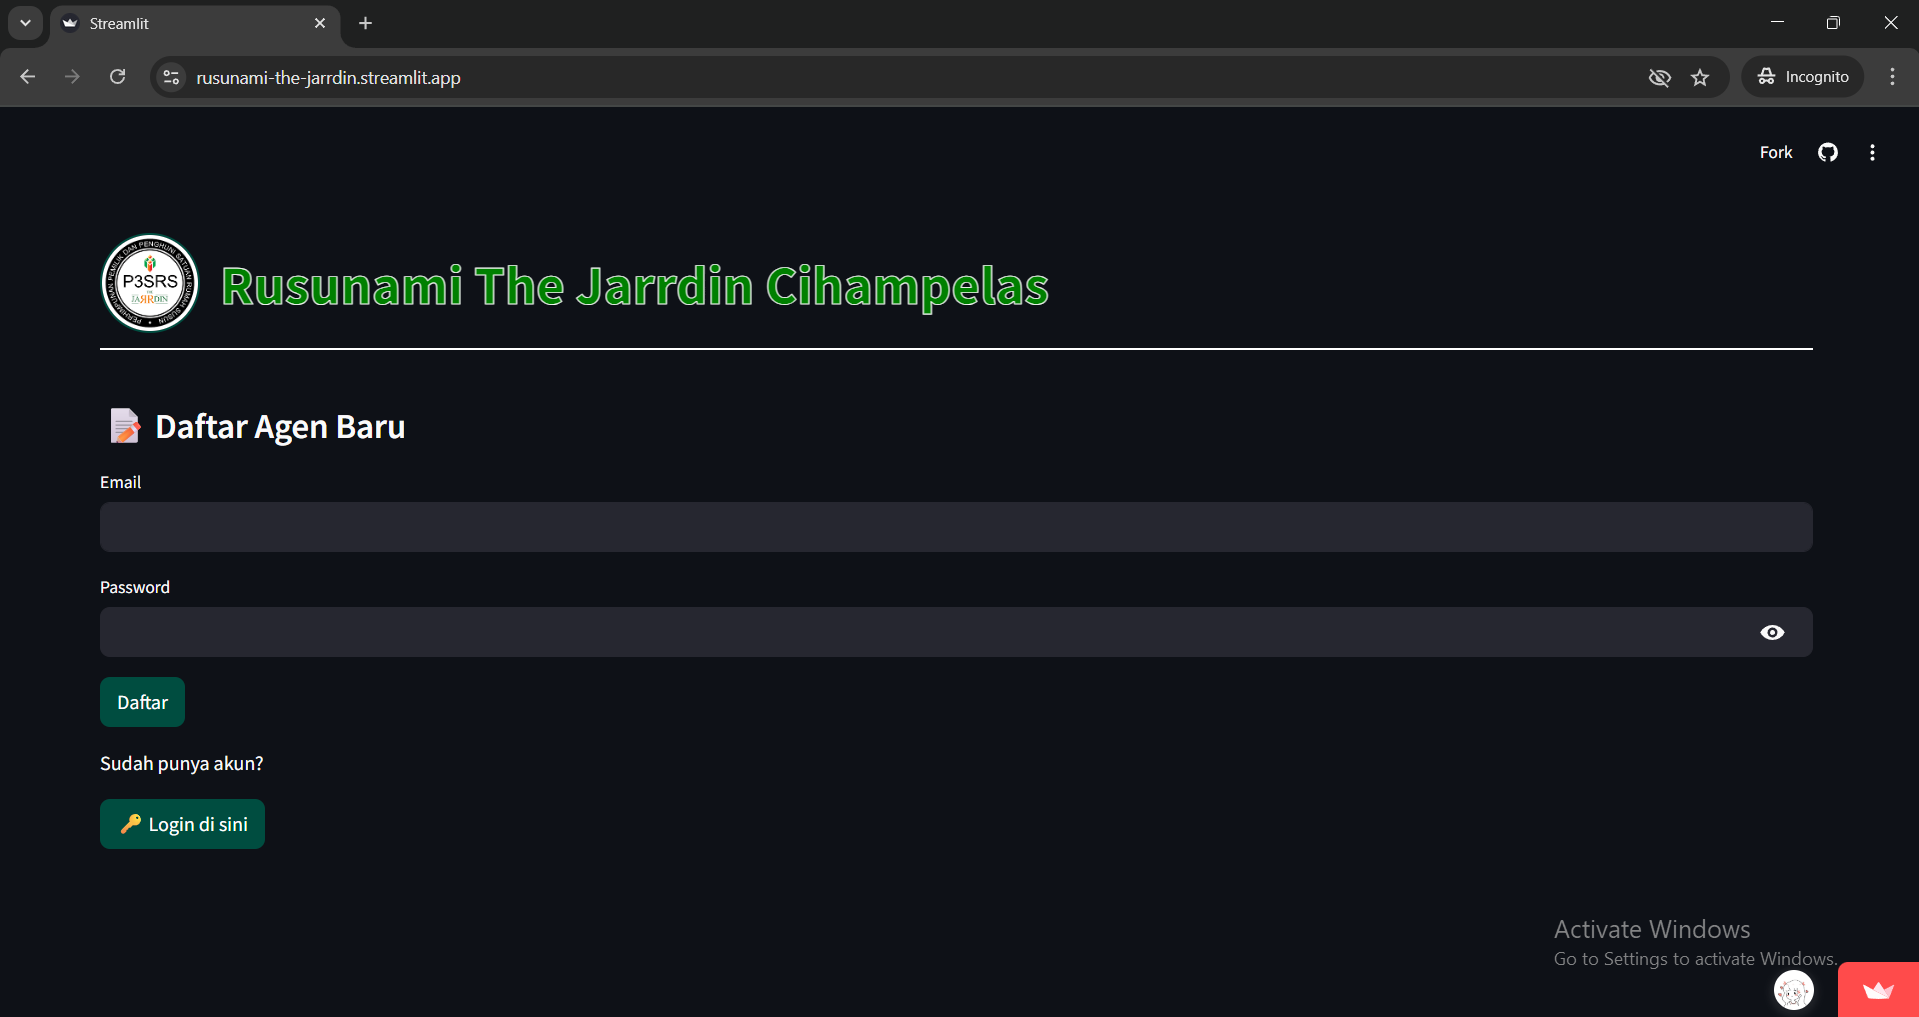
\includegraphics[width=0.7\textwidth]{Gambar/halaman daftar.png}
        \caption{Halaman untuk Daftar}
        \label{fig:daftar}
    \end{figure}

    \begin{figure}[H]
        \centering
        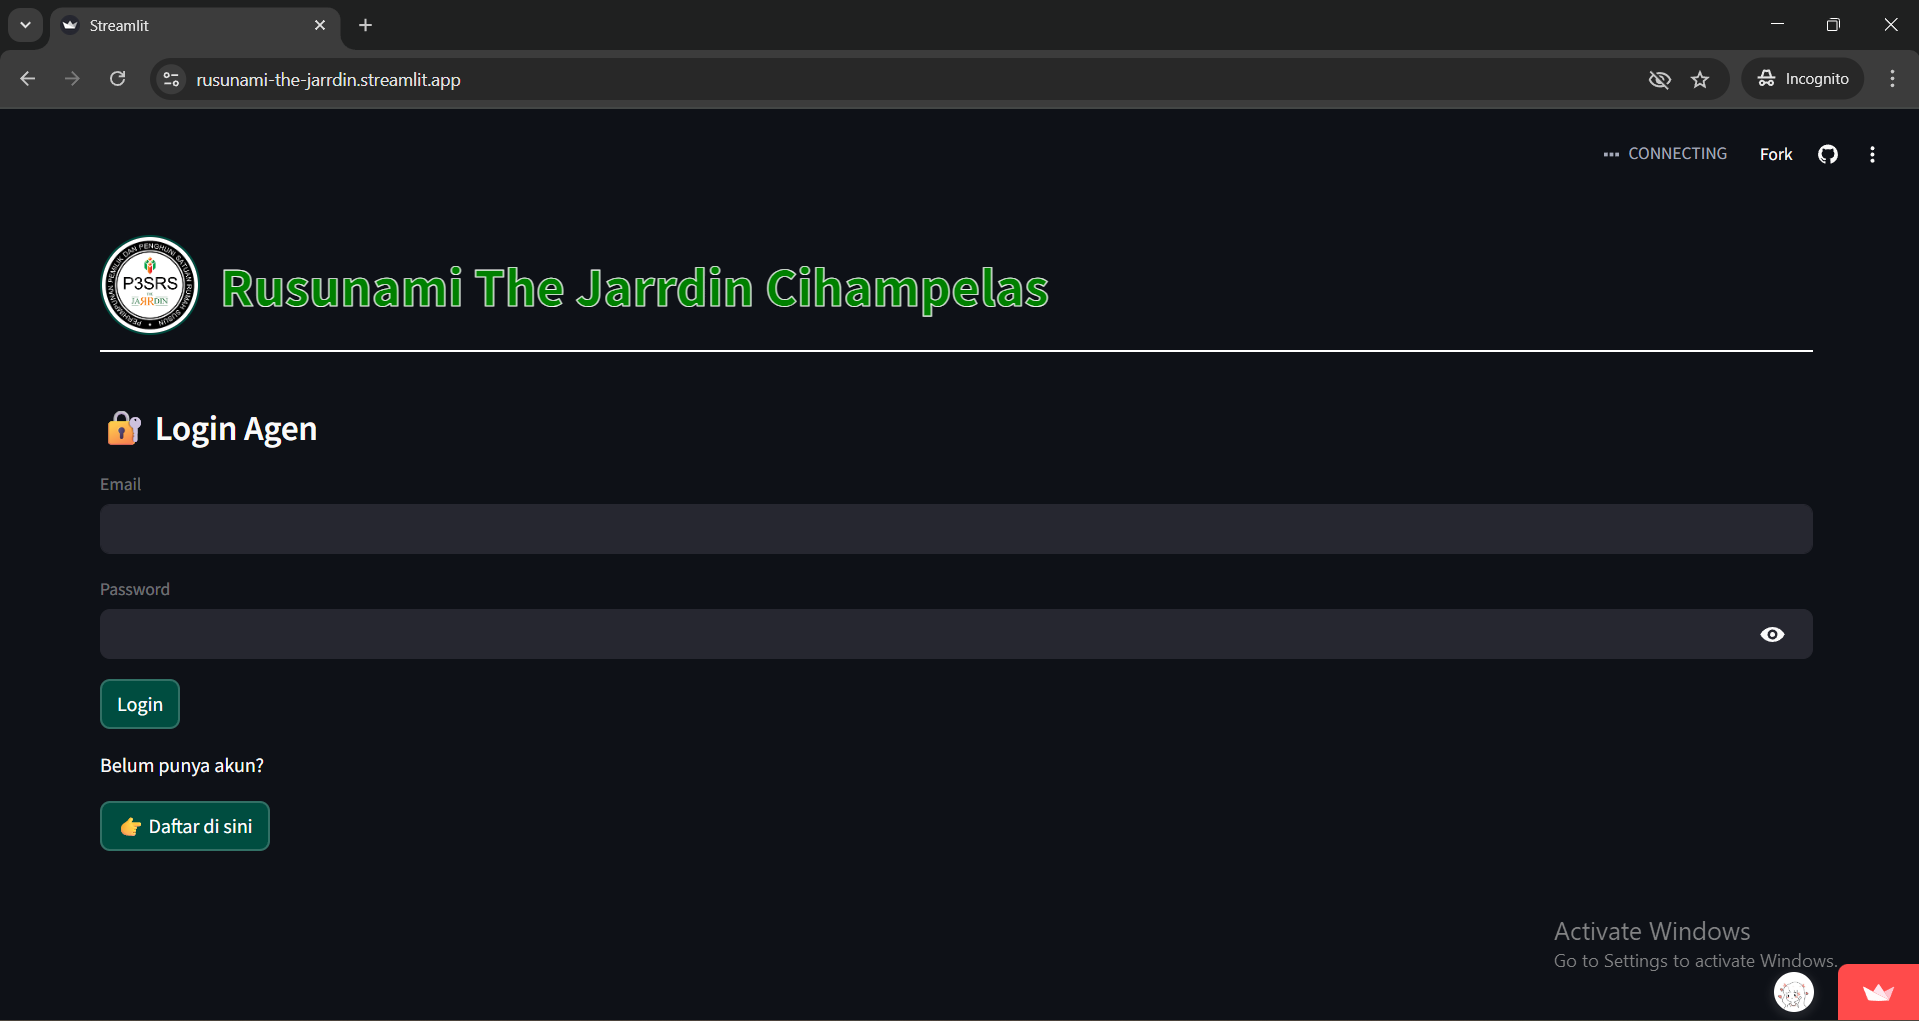
\includegraphics[width=0.7\textwidth]{Gambar/halaman login.png}
        \caption{Halaman untuk Login}
        \label{fig:login}
    \end{figure}

    Berikut adalah tangkapan layar halaman untuk melakukan input data penyewa. Akan muncul notifikasi ``\textit{Selamat datang, \texttt{user}}'' yang ditampilkan selama 10 detik. Selain itu, pada sisi kanan layar terdapat \textit{sidebar} yang berisi alamat email pengguna yang sedang masuk, menu, dan tombol \textit{logout} yang muncul setelah proses \textit{login} berhasil.

    \begin{figure}[H]
        \centering
        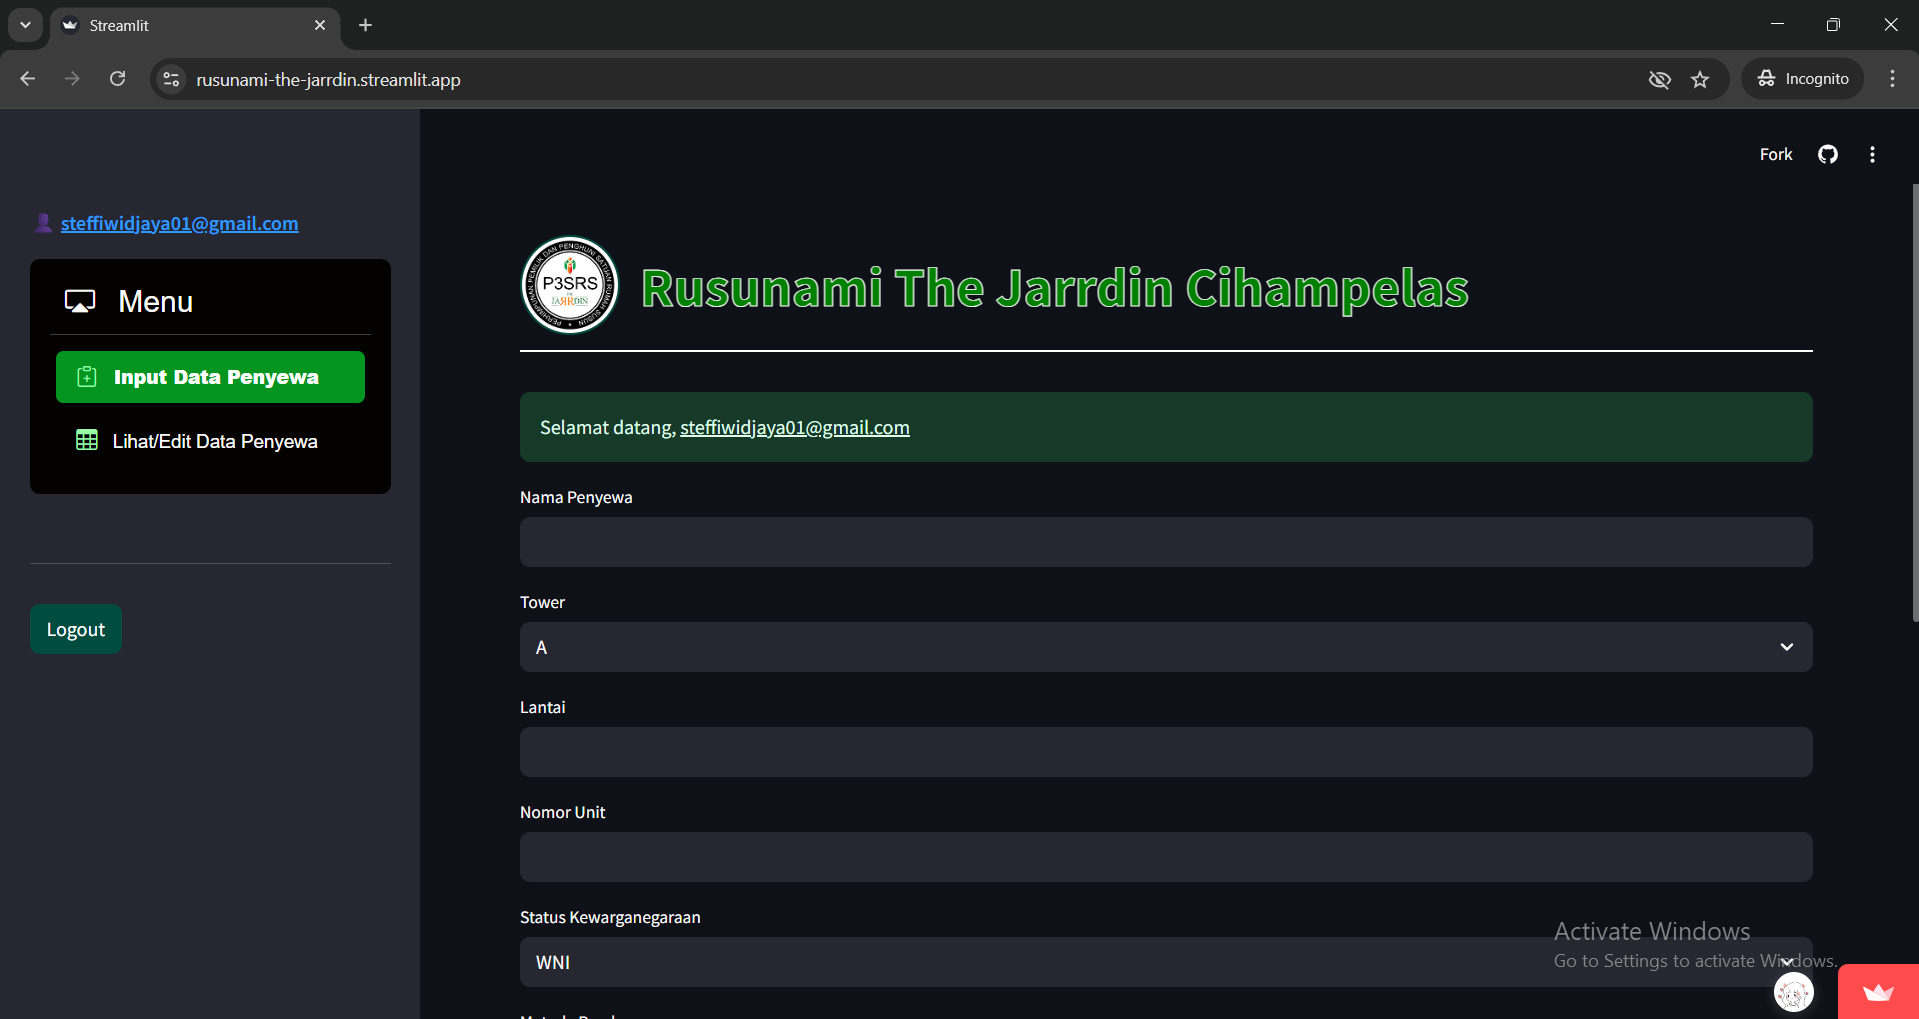
\includegraphics[width=0.7\textwidth]{Gambar/halaman input 1.png}
        \caption{Halaman untuk Input Data Penyewa}
        \label{fig:input1}
    \end{figure}

    \begin{figure}[H]
        \centering
        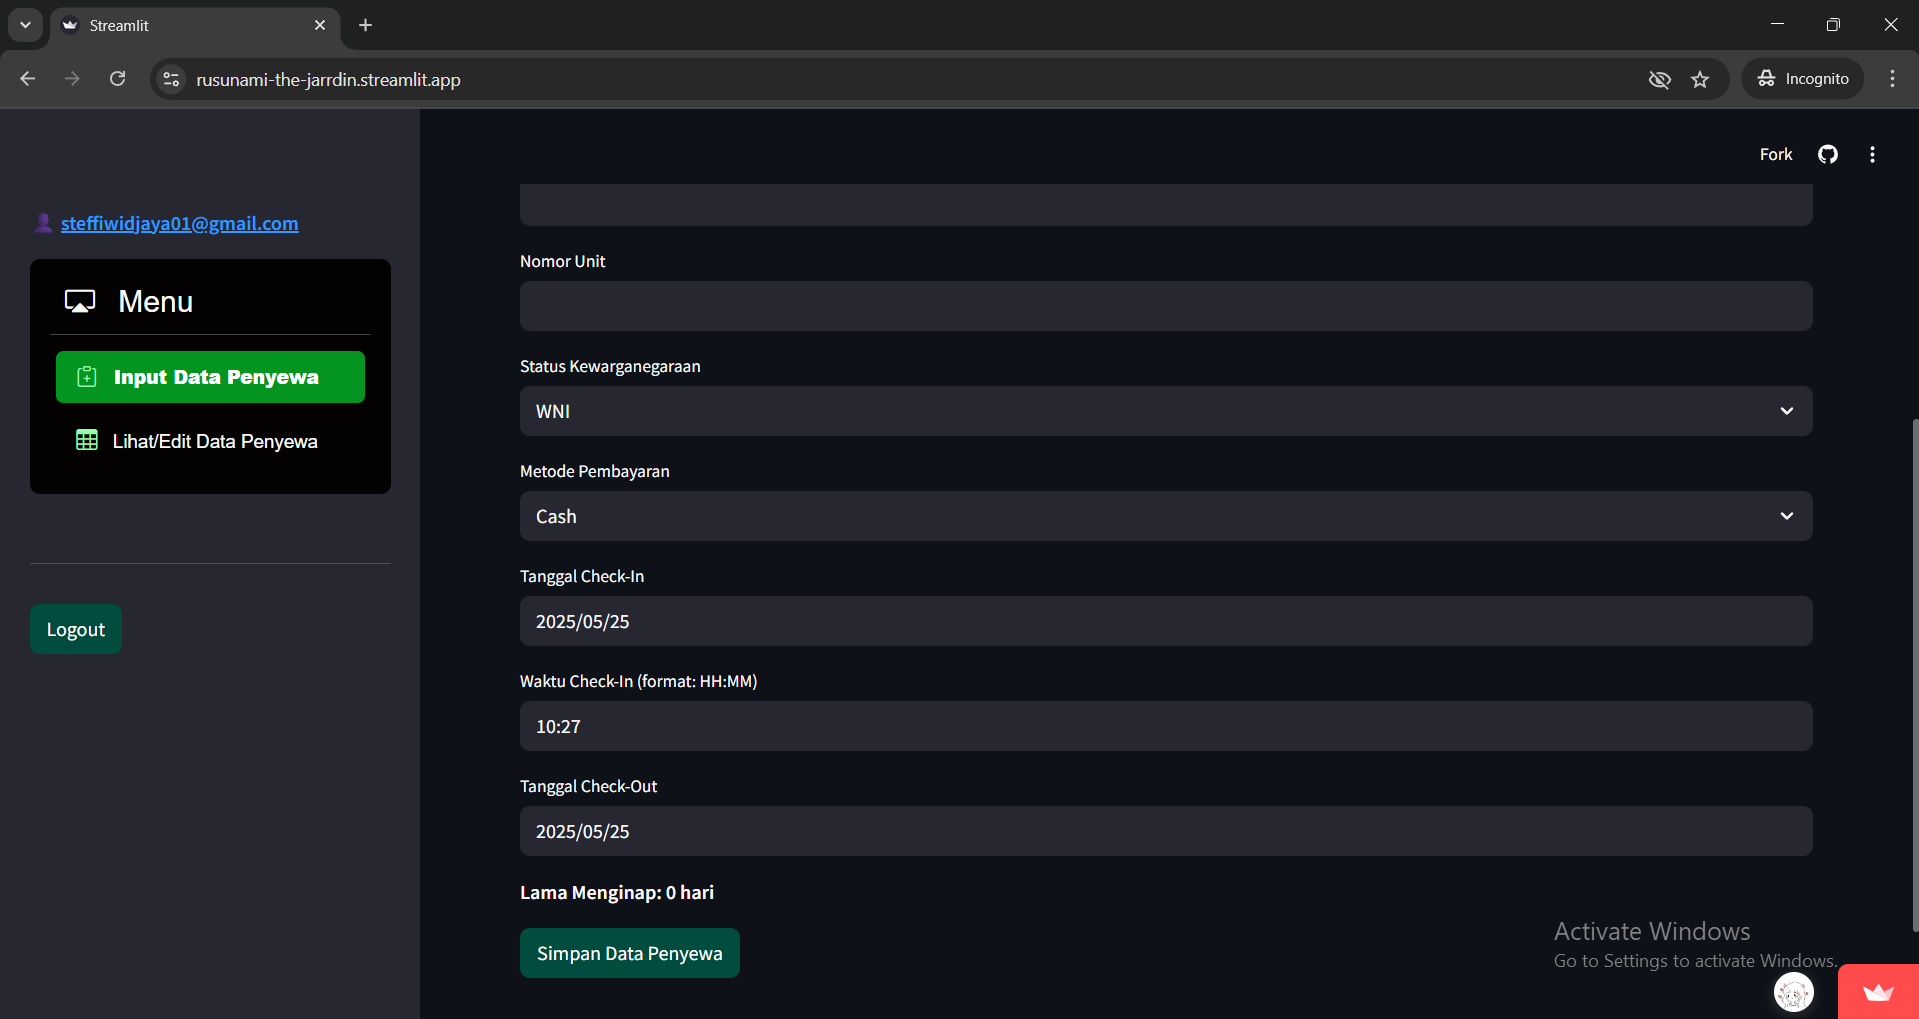
\includegraphics[width=0.7\textwidth]{Gambar/halaman input 2.png}
        \caption{Lanjutan Halaman Input Data Penyewa}
        \label{fig:input2}
    \end{figure}

    Berikut adalah tangkapan layar halaman untuk melihat atau mengedit data penyewa. Pada halaman ini, pengguna dapat melakukan \textit{refresh table} apabila baru saja melakukan pengeditan data (seperti mengisi waktu \textit{check-out} atau menambahkan komentar pelanggaran sewa) dan ingin melihat data tabel yang telah diperbarui.
    
    \begin{figure}[H]
        \centering
        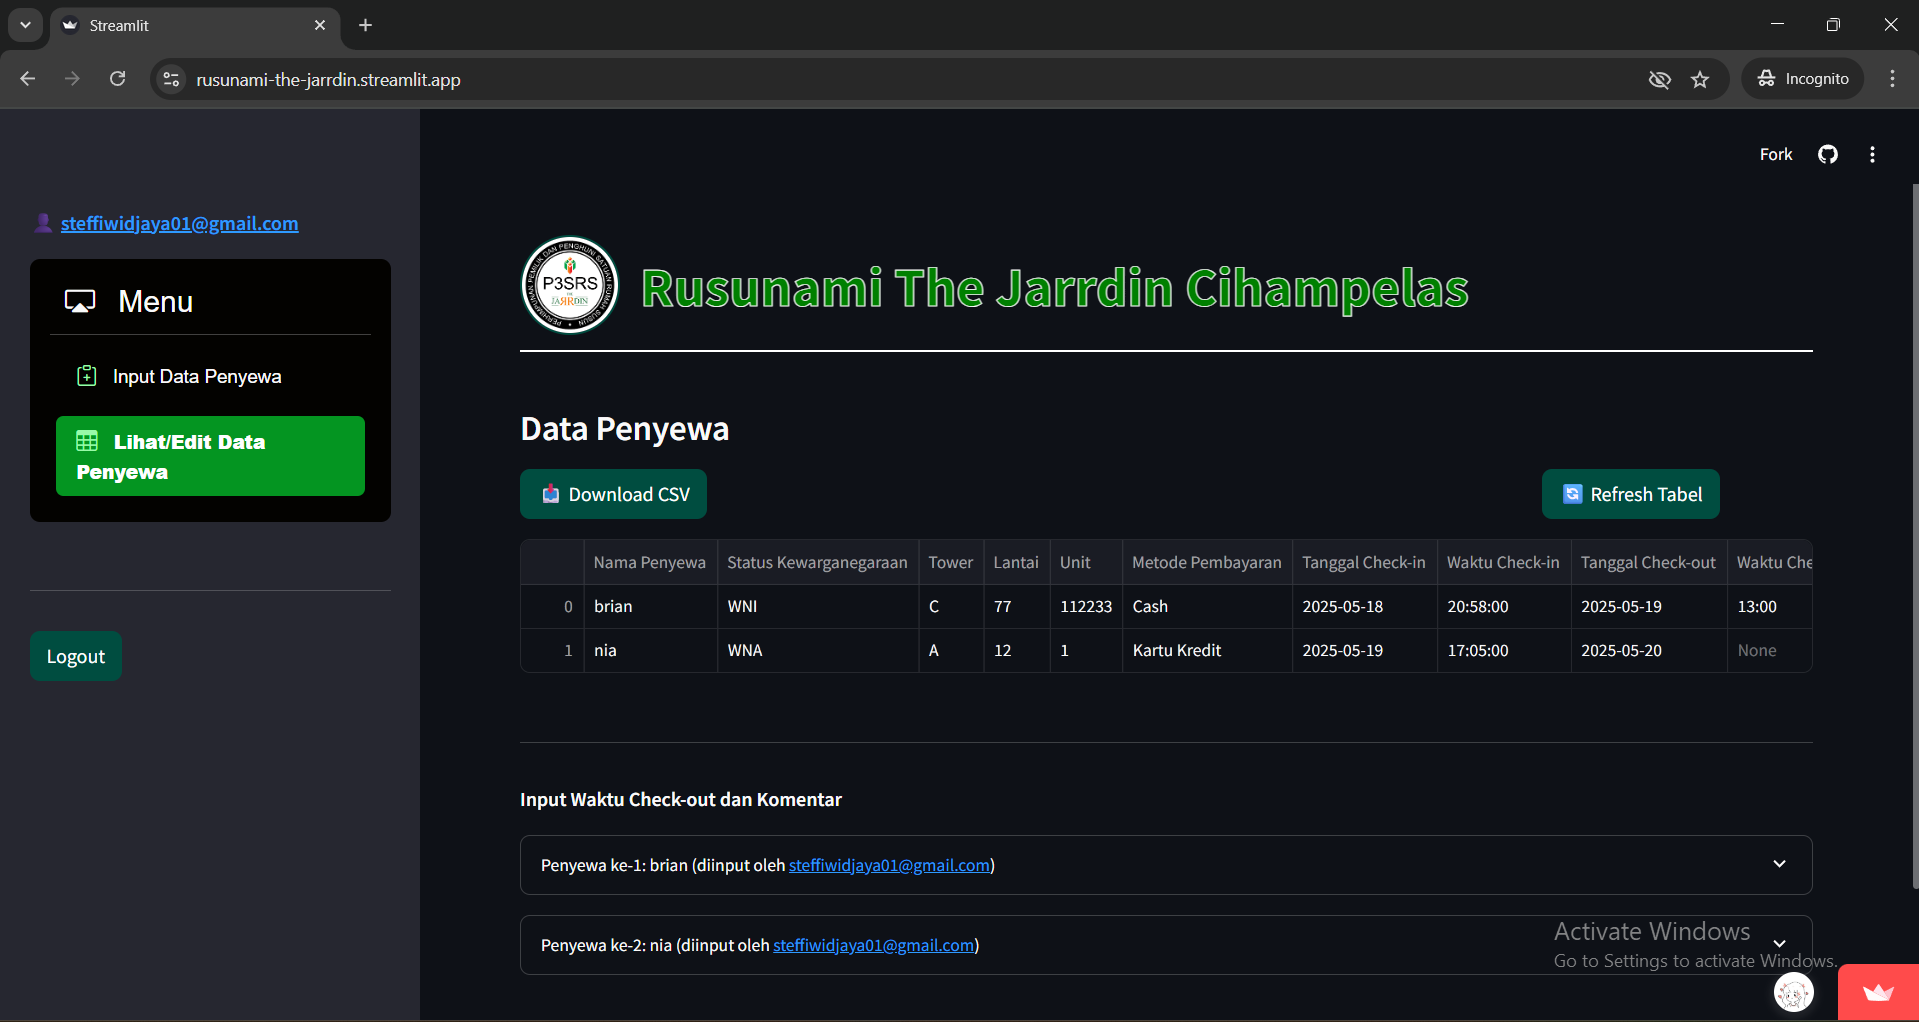
\includegraphics[width=0.7\textwidth]{Gambar/halaman lihat or edit (lihat).png}
        \caption{Halaman untuk Melihat atau Edit Data Penyewa}
        \label{fig:lihat_data}
    \end{figure}

    \begin{figure}[H]
        \centering
        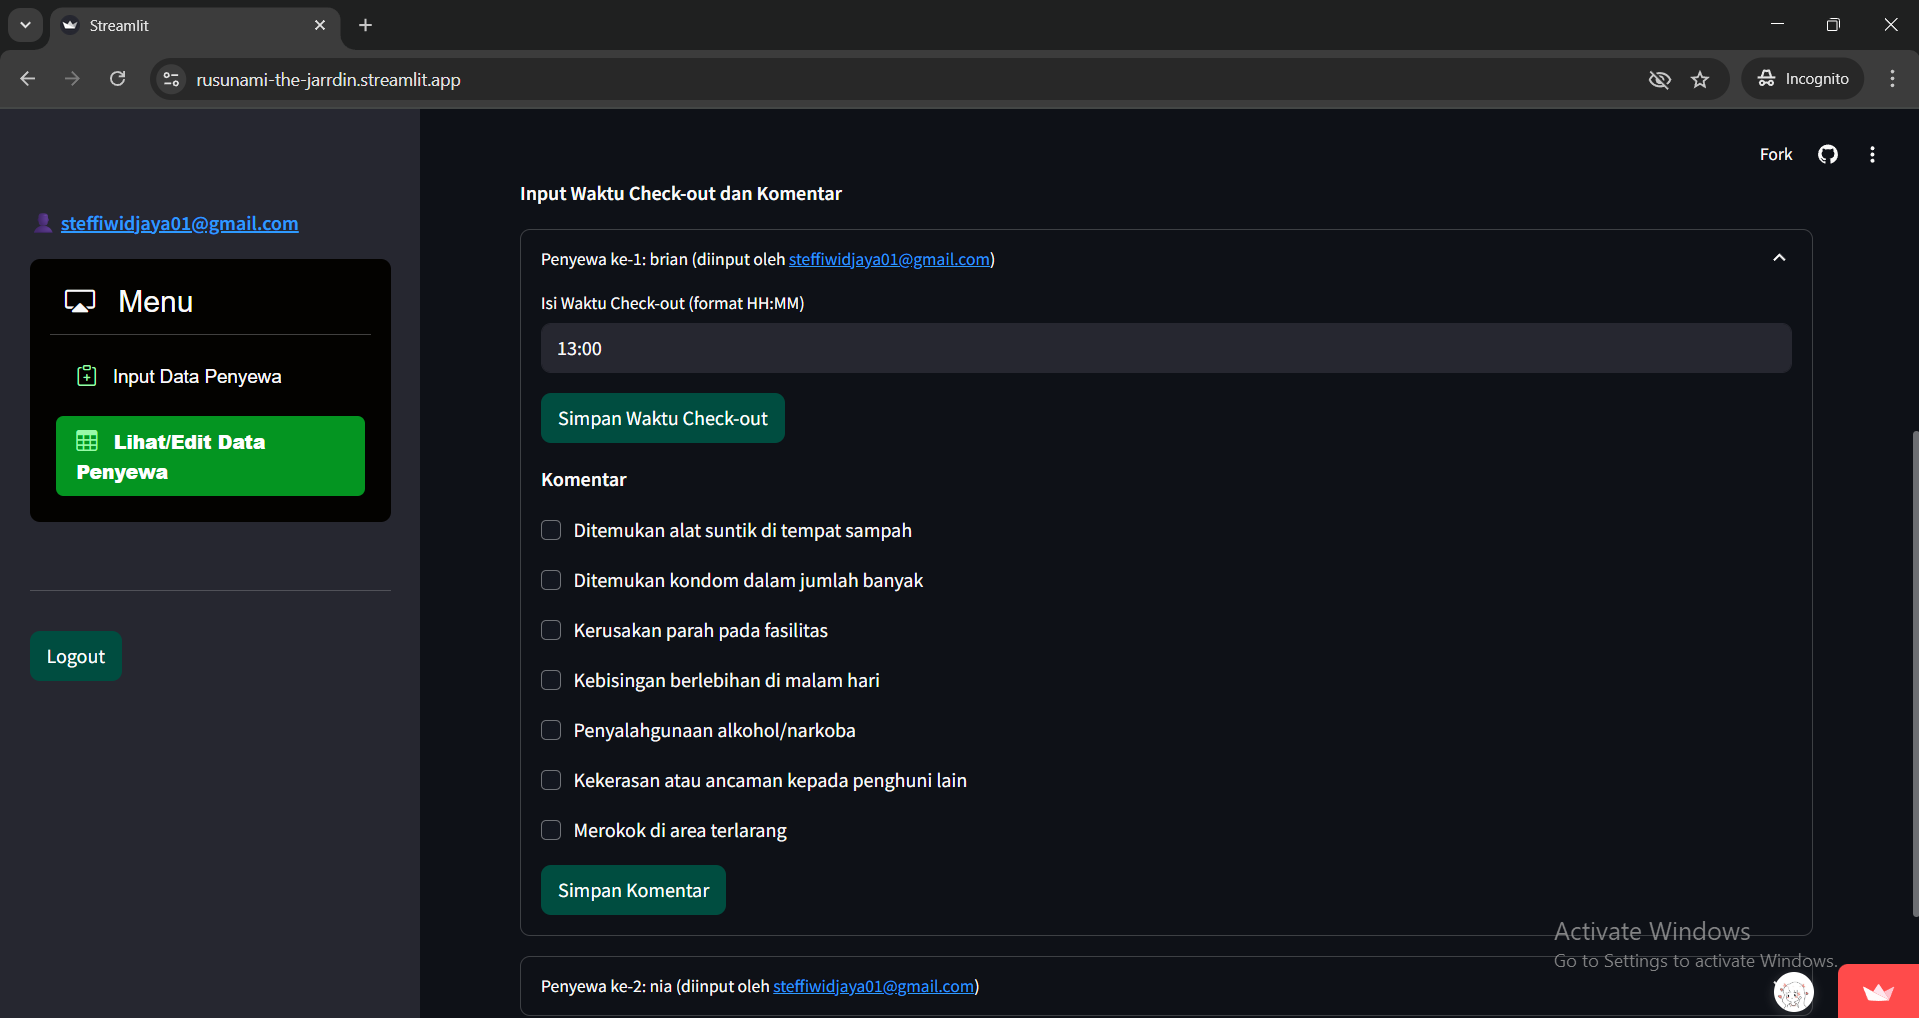
\includegraphics[width=0.7\textwidth]{Gambar/halaman lihat or edit 2 (edit).png}
        \caption{Lanjutan Halaman untuk Melihat atau Edit Data Penyewa}
        \label{fig:lihat_data2}
    \end{figure}

    \item \textbf{Keputusan akhir (Node.js)} \\
    Berdasarkan saran dan arahan dari dosen pembimbing, pengembangan sistem \textit{backend} dan antarmuka web akhirnya diputuskan untuk menggunakan \textbf{Node.js}. Keputusan ini diambil dengan pertimbangan utama sebagai berikut.
    \begin{itemize}
        \item \textbf{Integrasi sistem}\\
        Penggunaan Node.js menjamin kompatibilitas penuh dan kemudahan integrasi dengan sistem \texttt{srusun.id} serta modul-modul lain yang dikembangkan oleh mahasiswa sepembimbing dalam lingkungan ekosistem Rusunami The Jarrdin Cihampelas (RTJC).
        \item \textbf{Keseragaman teknologi}\\\
        Menyamakan \textit{stack} teknologi dengan infrastruktur yang sudah ada mempermudah proses \textit{deployment} dan pemeliharaan sistem di masa mendatang.
    \end{itemize}
\end{enumerate}

Meskipun sistem utama dibangun menggunakan Node.js, proses pengembangan dan pelatihan model \textit{machine learning} tetap dilakukan menggunakan Python karena keunggulan pustakanya. 


% tambahkan UI dari awal sampai yg final
